\section{实验验证与分析}\label{sec:exp}

本节介绍了所使用的数据集以及评价指标。接下来的小节详细描述了相关消融实验。最后展示实验结果并与相关文献进行对比分析。

\subsection{数据集}
实验在LM-O\cite{lmo}、YCB-V\cite{ycbv}和T-LESS\cite{tless}数据集上进行。这些数据集涵盖了广泛的场景,包括严重遮挡、纹理缺失和具有对称的物体。LM-O数据集包含8个家用弱纹理物体。YCB-V数据集由21个物体组成,包括有纹理和无纹理的物体。T-LESS数据集为工业物体模型数据集,包含30个工业物体,模型不包含模型的纹理,渲染的仿真图像也不包含真实纹理。

BOP挑战赛\cite{Sundermeyer2023BOPC2}使用这些数据集提供的物体模型,针对每个数据集生成五万张基于物理渲染(Physically-Based Rendering,PBR)合成图像。本研究采用这些PBR图像进行训练,但在数据集提供的真实场景中进行测试。

\subsection{评价指标}\label{subsec:评价指标}

\par 对于LM-O数据集,使用ADD与ADD-S指标进行评测,这是该数据集上常用的指标之一。ADD计算物体坐标系坐标分别用估计位姿和真实位姿投影到相机坐标系,计算对应投影点间距离在阈值内的百分比。其公式为:
\begin{equation}
  \text{ADD} = \frac{1}{n}\sum_{x_i \in M} \| (R_{gt}x_i + t_{gt}) - (R_{est}x_i + t_{est}) \|
\end{equation}
其中,$M$为物体的3D模型点集,$R_{gt}$和$t_{gt}$为真实位姿的旋转和平移,$R_{est}$和$t_{est}$为估计位姿的旋转和平移。

\par 对于对称物体,通常采用ADD-S,ADD-S指标与ADD指标的不同之处在于匹配估计位姿和真实位姿间距离时,需要寻找最近的模型点而不是完全相同的模型点。其公式为:
\begin{equation}
  \text{ADD-S} = \frac{1}{n}\sum_{x_i \in M} \min\limits_{x_j \in M} \| (R_{gt}x_i + t_{gt}) - (R_{est}x_j + t_{est}) \|
\end{equation}
通常对于非对称物体,选择用ADD指标,对于对称物体,选用ADD-S指标。这种混合指标的平均值称为ADD-(S)指标。

\par 此外,为了确定有多少概率能够实现网络输出的精度达到要求,对于ADD、ADD-S以及ADD-(S)会设定阈值。阈值的计算通常有两种方式,一种为固定数值,例如10厘米,另一种为与物体直径成比例关系,例如0.1d表示阈值设定为物体直径的$10\%$。对于YCB-V数据集,还计算ADD(-S)在不同阈值的曲线下面积(AUC),最大阈值为10厘米,如文献\cite{ycbv}所述。

\par 此外,对于这两个数据集,还对比了BOP挑战赛定义的BOP评价指标\cite{Sundermeyer2023BOPC2}。该评估采用三个指标:可见表面差异(Visible Surface Discrepancy,VSD)、最大对称感知表面距离(Maximum Symmetry-Aware Surface Distance,MSSD)和最大对称感知投影距离(Maximum Symmetry-Aware Projection Distance,MSPD)。VSD通过仅考虑物体的可见部分,将不可区分的位姿视为等效。该指标通过比较估计位姿和真实位姿下物体模型的可见表面,评估两者之间的差异。MSSD考虑了一组预先识别的全局物体对称性,通过测量3D空间中物体表面的偏差来评估位姿的准确性。MSPD同样考虑物体的对称性,但通过测量物体在图像平面上的可感知偏差来评估位姿的准确性。这三个指标的召回率平均值,称为AR,作为整体性能指标。

\par VSD的计算公式为:
\begin{equation}
e_\mathrm{VSD}\big(\hat{D}, \bar{D}, \hat{V}, \bar{V}, \tau\big) =
\mathrm{avg}_{\bm{p} \in \hat{V} \cup \bar{V}}
\begin{cases}
0 & \text{如果 } \bm{p} \in \hat{V} \cap \bar{V} \text{且 } \big|\hat{D}(\bm{p}) - \bar{D}(\bm{p})\big| < \tau \\
1 & \text{否则}
\end{cases}
\end{equation}
其中,$\hat{D}$ 和 $\bar{D}$ 表示通过渲染物体模型 $M$ 在估计位姿 $\hat{P}$ 和真实位姿 $\bar{P}$ 下得到的距离图。将这些距离图与测试图像 $I$ 的距离图 $D_I$ 进行比较,得到可见性掩码 $\hat{V}$ 和 $\bar{V}$,即模型 $M$ 在图像 $I$ 中可见的像素集合。参数 $\tau$ 表示错位容忍度。

\par MSSD的计算公式为:
\begin{equation}
e_{\text{MSSD}}\big(\hat{\bm{P}}, \bar{\bm{P}}, S_M, V_M\big) = \min_{\bm{S} \in S_M} \max_{\bm{x} \in V_M}
\big\Vert \hat{\bm{P}}\bm{x} - \bar{\bm{P}}\bm{S}\bm{x} \big\Vert_2
\end{equation}
其中,$S_M$ 是物体模型 $M$ 的全局对称变换集合,$V_M$ 是模型顶点的集合,2-范数$\big\Vert \cdot \big\Vert_2$表示距离。

\par MSPD的计算公式为:
\begin{equation}
e_{\text{MSPD}}\big(\hat{\bm{P}}, \bar{\bm{P}}, S_M, V_M\big) = \min_{\bm{S} \in S_M} \max_{\bm{x} \in V_M}
\big\Vert \text{proj}\big( \hat{\bm{P}}\bm{x} \big) - \text{proj}\big( \bar{\bm{P}}\bm{S}\bm{x} \big) \big\Vert_2
\end{equation}
函数 $\text{proj}(\cdot)$ 表示二维投影(结果以像素为单位),其他符号的含义与 MSSD 中相同。

\subsection{与现有方法进行比较}
本小节对多个通用数据集上的实验结果与现有方法进行了比较。

\begin{table}
  \centering
  \resizebox{\textwidth}{!}{%
  \begin{tabular}{c|c|c|c|c|c|c|c}
    \toprule 
    \multirow{2}{*}{方法} & \multicolumn{2}{c|}{RGB 输入方法} & \multicolumn{5}{c}{RGB-D 输入方法} \\ 
         \cline{2-8}
      & GDR-Net\cite{wang2021gdr} 
& ZebraPose\cite{su2022zebrapose}&  PR-GCN\cite{Zhou2021PRGCNAD} 
&  FFB6D\cite{he2021ffb6d} 
& RCVPose\cite{wu2022vote} 
& DFTr\cite{zhou2023deep} &本文方法\\
    \midrule
     ape & 46.8 
& 57.9& 40.2 
& 47.2 
&  60.3 
& 64.1 &  \textbf{78.0}\\
     can & 90.8 
& 95.0& 76.2 
& 85.2 
&  92.5 
& 96.1 &  \textbf{98.9}  \\
     cat & 40.5 
& 60.6& 57.0 
& 45.7 
&  50.2 
& 52.2 &  \textbf{87.5}\\
     driller & 82.6 
& 94.8& 83.2 
& 81.4 
&  78.2 
& 95.8 &  \textbf{97.8}\\
     duck & 46.9 
& 64.5& 30.0 
& 53.9 
&  52.1 
& 72.3 &  \textbf{85.3}\\
     eggbox* & 54.2 
& 70.9& 68.2 
& 70.2 
&  \textbf{81.2} 
& 75.3 &  80.3\\
     glue* & 75.8 
& 88.7& 67.0 
& 60.1 
&  72.1 
& 79.3 &  \textbf{94.1}\\
     holepuncher & 60.1 
& 83.0& \textbf{97.2} 
& 85.9 
& 75.2 
& 86.8 &  95.2  \\
     \hline
     均值 & 62.2 & 76.9&  65.0 &  66.2 &  70.2 & 77.7 & \textbf{89.6}\\
    \bottomrule
  \end{tabular}
  }
  \caption{LM-O数据集上ADD-S对比结果}
  \label{tab:lmo_results_table_}
\end{table}



\textbf{LM-O数据集上的结果 } 在\autoref{tab:lmo_results_table_}中,HiPose与现有方法在LM-O数据集上的ADD(-S)评分进行了比较。使用了CDPN\cite{li2019cdpn}提供的2D检测结果,该检测器基于FCOS\cite{fcos}进行训练,且仅使用BOP挑战赛提供的PBR图像进行训练。结果表明,HiPose相比于最好的RGB-D方法DFTr高出$11.9\%$,相比于最好的仅使用RGB的方法ZebraPose高出$12.7\%$,表现优异。

\begin{table}
  \centering
  \caption{YCB-V数据集上AUC对比结果}
  \label{tab:ycbv_results_table}
  \resizebox{0.3\textwidth}{!}{%
  \begin{tabular}{@{}l|c|c|c@{}}
    \toprule
     \multicolumn{2}{c|}{方法} & \makecell{AUC of\\ADD-S} & \makecell{AUC of\\ADD(-S)} \\
    \midrule
    \multirow{3}{*}{\rotatebox{90}{RGB}} & SO-Pose~\cite{Di_2021_ICCV} &  90.9 &  83.9  \\
     & GDR-Net~\cite{wang2021gdr} &  91.6 &  84.4 \\
     & ZebraPose~\cite{su2022zebrapose} & 90.1 & 85.3\\
     \midrule
    \multirow{5}{*}{\rotatebox{90}{RGB-D}} & PVN3D~\cite{he2020pvn3d} &  95.5 &  91.8 \\
     & RCVPose~\cite{wu2022vote} &  96.6 &  95.2 \\
     & FFB6D~\cite{he2021ffb6d} &  96.6 &  92.7 \\
     & DFTr~\cite{zhou2023deep} & 96.7 & 94.4\\
     & 本章方法 &  \textbf{97.6} &  \textbf{95.5}  \\
    \bottomrule
  \end{tabular}
  }
\end{table}


\textbf{YCB-V数据集上的结果 } 在\autoref{tab:ycbv_results_table}中,HiPose与现有方法在YCB-V数据集上的ADD和ADD-S评分进行了比较。所有其他方法在训练中均使用了真实和合成图像。为了公平比较,此处使用的2D FCOS检测器也在真实和合成图像上进行了训练。结果表明,HiPose在YCB-V数据集上的表现再次超越了所有其他方法,具有显著的优势(约$1\%$的提升)。考虑到YCB-V数据集的评分已经接近饱和,这一结果尤为突出。

\autoref{tab:ycbv_full_results_AUC}总结了YCB-V数据集上每个物体的结果。如表所示,大多数测试物体上的性能优于其他方法。展示了ADD(-S)和ADD-S的AUC的平均召回率(以百分比表示),并与现有方法进行了比较。(*)表示对称物体。

\begin{table}
  \centering
  \caption{在BOP挑战赛上的对比结果}
  \label{tab:bop_score_table}
  \resizebox{\textwidth}{!}{%
  \begin{tabular}{l|c|c|c|c|c|c|c}
    \toprule
     方法 & 训练数据 & 后优化方法 & LM-O & YCB-V & T-LESS & AR & 时间(秒) \\
    \midrule
    FFB6D-CVPR21-PBR-NoRefinement\cite{he2021ffb6d} & PBR &  - & 68.7 &  75.8  & - & 72.3$^*$ & 0.19$^*$\\
    RCVPose 3D\_SingleModel\_VIVO\_PBR\cite{wu2022vote} & PBR &  ICP~\cite{Rusinkiewicz2001EfficientVO} & 72.9 &  84.3  & 70.8 & 76.0 & 1.33\\
    SurfEmb-PBR-RGBD\cite{haugaard2022surfemb} & PBR & custom\cite{haugaard2022surfemb} & 76.0 &  79.9  & 82.8 & 79.6 & 9.04\\
    RADet+PFA-PBR-RGBD\cite{Hai2023RigidityAwareDF} & PBR &  PFA~\cite{hu2022perspective} & 79.7 &  82.6  & 80.2 & 80.8 & 2.63\\
    GDRNPP-PBR-RGBD-MModel\cite{wang2021gdr} & PBR &  $\sim$CIR~\cite{lipson2022coupled} & 77.5 &  90.6  & \textbf{85.2} & 84.4 & 6.37\\
    HiPose (本章) & PBR &  - & \textbf{79.9} &  \textbf{90.7}   & 83.3 & \textbf{84.6} & \textbf{0.16}\\
    \bottomrule
  \end{tabular}
  }
\end{table}


\begin{table}[ht]
    \centering
    \caption{各物体在YCB-V数据集上的结果}
    \label{tab:ycbv_full_results_AUC}
    \resizebox{\textwidth}{!}{%
    \begin{tabular}{@{}l|c|c|c|c|c|c|c|c@{}}
      \toprule 
       方法 & \multicolumn{2}{c|}{PVN3D\cite{he2020pvn3d}} & \multicolumn{2}{c|}{FFB6D\cite{he2021ffb6d}} &  \multicolumn{2}{c|}{DFTr\cite{zhou2023deep}} &  \multicolumn{2}{c}{\textbf{本章方法}}\\
      \midrule
      指标 & \makecell{AUC of ADD-S} & \makecell{AUC of ADD(-S)} &\makecell{AUC of ADD-S} & \makecell{AUC of ADD(-S)} & \makecell{AUC of ADD-S} & \makecell{AUC of ADD(-S)} & \makecell{AUC of ADD-S} & \makecell{AUC of ADD(-S)} \\ 
      \midrule
       002\_master\_chef\_can & 96.0&  80.5&  96.3& 80.6& \textbf{97.0}& \textbf{92.3}      & 96.4	&86.2\\
       003\_cracker\_box      & 96.1&  94.8&  96.3& 94.6 &95.9 &93.9         & \textbf{97.7}&	\textbf{96.7}\\
       004\_sugar\_box        & 97.4&  96.3&  97.6& 96.6& 97.1& 95.5       & \textbf{98.2}&	\textbf{97.1}\\
       005\_tomato\_soup\_can & 96.2&  88.5 & 95.6& 89.6& 95.6& 92.6      & \textbf{97.0}	&\textbf{95.1}\\
       006\_mustard\_bottle   & 97.5&  96.2 &  97.8& \textbf{97.0}& 97.6& 96.3           & \textbf{98.4}&	96.9\\
       007\_tuna\_fish\_can   & 96.0&  89.3& 96.8 &88.9 &97.3 &94.5           & \textbf{97.8}&	\textbf{96.2}\\
       008\_pudding\_box      & 97.1 &  95.7& 97.1 &94.6 &97.4 &95.7       & \textbf{98.8}&	\textbf{98.1}\\
       009\_gelatin\_box      & 97.7&  96.1&  98.1 &96.9 &97.6& 96.3           & \textbf{98.9}	&\textbf{97.8}\\
       010\_potted\_meat\_can & 93.3 &  88.6&  94.7& 88.1& \textbf{95.9}& \textbf{92.1}         & 93.5	&83.4\\
       011\_banana            & 96.6 &  93.7&  97.2 &94.9 &97.1 &95.0          & \textbf{98.6}&	\textbf{96.3}\\
       019\_pitcher\_base     & 97.4&  96.5& \textbf{97.6}& \textbf{96.9}& 96.0& 93.1           & 96.8	&93.2\\
       021\_bleach\_cleanser  & 96.0&  93.2& 96.8 &94.8& 96.8& \textbf{94.9}            &\textbf{97.1}&	94.0\\
       024\_bowl*             & 90.2 &  90.2& 96.3& 96.3& 96.9& 96.9           &\textbf{98.0}	&\textbf{98.0}\\
       025\_mug               & 97.6&  95.4& 97.3& 94.2& 97.6& 94.9         & \textbf{98.2}	&\textbf{95.7}\\
       035\_power\_drill      & 96.7&  95.1& 97.2& 95.9& 96.9& 95.2           & \textbf{98.3}&	\textbf{97.4}\\
       036\_wood\_block*      & 90.4&  90.4& 92.6& 92.6& 96.2& 96.2           & \textbf{97.0}	&\textbf{97.0}\\
       037\_scissors          & 96.7&  92.7& 97.7& 95.7& 97.2& 93.3            &\textbf{98.3}&	\textbf{96.8}\\
       040\_large\_marker     & 96.7&  91.8& 96.6& 89.1& 96.9 &92.7          & \textbf{98.6}	&\textbf{94.3}\\
       051\_large\_clamp*     & 93.6&  93.6&  \textbf{96.8}& \textbf{96.8}& 96.3 &96.3          & 95.9&	95.9\\
       052\_extra\_large\_clamp* & 88.4&  88.4& 96.0& 96.0 &\textbf{96.4}& \textbf{96.4}         & 95.6&	95.6\\
       061\_foam\_brick*          & 96.8&  96.8& 97.3& 97.3& 97.3 &97.3       & \textbf{98.6}	&\textbf{98.6}\\
       \hline
       均值 & 95.5&  91.8&  96.6 &92.7& 96.7 &94.4             &\textbf{97.5} &\textbf{95.3} \\
      \bottomrule
    \end{tabular}
    }
\end{table}

\textbf{BOP挑战赛上的结果 } \autoref{tab:bop_score_table}展示了所有仅在PBR仿真合成数据下训练的结果,($\sim$) 表示类似于 CIR\cite{lipson2022coupled}。$^*$ 仅在 LM-O 和 YCB-V 上取平均,因为该方法未提供 T-LESS 的结果。 BOP挑战赛提供了更公平的比较平台,提供了统一的训练数据集和标准2D检测结果,以及更具信息量的评价指标\cite{hodan2018bop}。本章方法使用了BOP挑战赛2023提供的默认检测结果。

大多数在\autoref{tab:bop_score_table}中的方法依赖于耗时的基于渲染的位姿优化步骤,而HiPose无需任何渲染对比过程即可直接估计出精确的物体位姿。HiPose在LM-O和YCB-V数据集上超越了现有方法,并在T-LESS数据集上取得了与领先方法非常接近的结果。综合考虑三个数据集的平均召回率,HiPose的召回率高于所有其他方法。

GDRNPP\cite{liu2022gdrnpp_bop} 的结果与 HiPose 最为接近,但 HiPose 的速度约为 GDRNPP(包含优化步骤)的 $40$ 倍。这表明 HiPose 既准确又计算高效。

\subsection{消融实验}

本小节通过多项消融实验和分析全面探讨 HiPose 在不同设计选择下的表现,分析不同参数的影响以及各模块在算法中的作用。所有消融实验均在LM-O数据集上完成,\autoref{tab:hipose_ablation_study} 汇总了不同实验设置下的结果,结果以ADD(-S)的平均召回率(\%)表示。

\begin{table}
  \centering
  \begin{tabular}{@{}c|c|c@{}}
    \toprule
     A0 &Kabsch& 86.65 \\
     A1 &RANSAC+ Kabsch& 89.12 \\
     A2 &Our Hierarchical Pruning &\textbf{89.62}\\
     \midrule
     B0 &Trust Bit Threshold 0.08& 89.55 \\
     B1 &Trust Bit Threshold 0.06& 89.61 \\
     B2 &Trust Bit Threshold 0.04& 89.59 \\
     \midrule
     C0 &Inlier Threshold: median $\rightarrow$ mean & 89.47 \\
     \midrule
     D0 & ConvNext-B~\cite{Liu2022ACF} $\rightarrow$ ResNet34~\cite{He2015DeepRL} & 88.64 \\
     \midrule
     E0 & ZebraPose(pbr)+RANSAC Kabsch&87.0\\
     E1 & ConcatRGBD+RANSAC Kabsch&84.5\\
    \bottomrule
  \end{tabular}
  \caption{在LM-O数据集上的消融实验}
  \label{tab:ablation_study}
\end{table}

\textbf{对应关系剪枝的有效性 }
在\autoref{tab:hipose_ablation_study}中,首先对比分层对应关系剪枝算法与Kabsch算法在精度上的区别。在A0实验中,直接使用Kabsch算法求解物体位姿。A2实验使用的是分层对应关系剪枝算法。结果表明A2实验的精度比直接使用Kabsch算法的ADD(-S)的平均召回率高$2.97\%$,验证了分层对应关系剪枝算法的有效性。该实验也说明了网络预测的二进制编码中存在少量离群值。

\begin{table}[htbp]
  \centering
  \caption{RANSAC+Kabsch 参数对A1实验ADD-(S)结果的影响}
  \label{tab:ablation_study_RANSAC_parameters}
  \begin{tabular}{@{}c|c|c|c|c|c|c@{}}
    \toprule
    对应关系数量  & 4 & 6 & 8 & 10 & 20 & 30 \\
     \midrule
     500 次迭代 & 88.7 & 89.0 & 89.0	& \textbf{89.1} & 89 & 88.7 \\
     1000 次迭代 & 89.0 & \textbf{89.1} & 88.9 & \textbf{89.1} & \textbf{89.1} & 88.8 \\
     1500 次迭代 & 89.0 & \textbf{89.1} & \textbf{89.1} & \textbf{89.1} & 88.9 & 88.8 \\
    \bottomrule
  \end{tabular}
\end{table}

将A1实验与A0实验进行比较,A1实验使用RANSAC框架识别离群值。实验结果表明,相对于A0的结果,A1的召回率提高了$2.47\%$。A1的结果受到若干超参数选择的影响,例如每次迭代中使用的对应关系数量、RANSAC迭代次数和每次迭代中的内点阈值等。此外,随机种子(seed)的变化对结果也有微弱的影响。此实验使用了Open3D\cite{zhou2018open3d}提供的RANSAC和Kabsch算法。
探索了多种参数组合,并展示了其中的最佳结果。在A1实验中,RANSAC+Kabsch方案通过Open3D库中的registration\_ransac\_based\_on\_correspondence函数实现。调整了每次RANSAC迭代中使用的对应关系数量和迭代次数,结果如\autoref{tab:ablation_study_RANSAC_parameters}所示。实验表明,尽管RANSAC+Kabsch方法能够提升一定的性能,但其效果仍不如分层对应关系剪枝方法。
调整了每次RANSAC迭代中的对应关系数量和RANSAC迭代次数,最大对应点对距离为2厘米。结果以ADD(-S)的平均召回率(\%)表示。根据表格,每次RANSAC迭代使用10个对应关系时效果最佳。然而,使用RANSAC+Kabsch方法得到的结果不如分层方法的结果。

与RANSAC方案A1相比,分层对应关系剪枝方案A2提供了稳定的结果,随机种子的选取对其影响更小。在实验A2中,第 $10$ 位被选择为初始位,并根据预测值高于$0.52$或低于$0.48$定义置信位。如\autoref{tab:hipose_ablation_study}所示,与不使用任何离群值策略A0相比,方法A2将召回率提高了$2.97\%$,同时超过了RANSAC可实现的最佳结果。

在\autoref{tab:ourlier_removal_metrics}中评估每次迭代中离群值移除的准确性,进一步显示对应关系剪枝的有效性。\autoref{tab:ourlier_removal_metrics}展示不同阈值下,网络估计的内点数量的精度和准确率。精度和准确率的提高证实了低质量对应关系的逐步移除。精度(Precision)指的是模型预测的正样本中实际为正样本的比例。精度越高,表示模型预测的正样本中错误的比例越低。准确率(Accuracy)指的是模型预测正确的样本占总样本的比例。准确率越高,表示模型整体预测的正确性越高。

\begin{table}[t]
  \centering
  \begin{tabular}{c|c|c|c|c|c|c|c|c}
    \toprule
    迭代步数 & 1 & 2 & 3 & 4 & 5 & 6 & 7 & 结果 \\
    \midrule
    精度 10mm (\%) & 66.1 &67.4 &70.3 &73.3 &73.8 &75.9 &75.9 &76.1\\
    精度 3mm (\%) & 14.3 &14.8 &16.0 &17.4 &17.6 &17.7 &17.7 &17.8\\
    准确率 3mm (\%)& 18.1 &22.6 &30.7 &36.9 &37.7 &38.5 &38.5 &39.5\\
    \bottomrule
  \end{tabular}
  \caption{不同迭代步骤下内点准确率和精度}
  \label{tab:ourlier_removal_metrics}
\end{table}


% % \vspace{-0.1cm}
% \begin{table}[t]
%   \centering
%   \scalebox{0.70}{
%   \begin{tabular}{c|c|c|c|c|c|c|c|c}
%     \toprule
%     Iteration Step & 1 & 2 & 3 & 4 & 5 & 6 & 7 & last \\
%     \hline
%     % Pre./Acc. & 14/18 &15/23 &16/31 &17/ 39&18/38 &18/39 &18/39 &18/39\\
%     precision & 0.143 &0.148 &0.160 &0.174 &0.176 &0.177 &0.177 &0.178\\
%     accuracy & 0.181 &0.226 &0.307 &0.369 &0.377 &0.385 &0.385 &0.395\\
%     \bottomrule
%   \end{tabular}
%   }
%   \label{tab:c}
% \end{table}
% % \vspace{-0.2cm}


% \begin{figure}[h]
% \begin{tikzpicture}
% \begin{axis}[
% scaled y ticks=real:1,
% ytick scale label code/.code={},
% yin = 0.10,
% ymax = 0.45,
% symbolic x coords={1, 2, 3, 4, 5, 6, 7, final},
% xtick=data,
% height=5cm,
% width=8cm,
% grid=major,
% xlabel={Iteration Step},
% ylabel={},
% y label style={at={(0.23,0.5)}},
% legend style={
%         at={(0.8,0.4)},
%         anchor=south,
%         legend columns=1,
%         nodes={scale=0.85, transform shape}
%     },
% ]
% \addplot coordinates {
% (1,0.143) 
% (2, 0.148) 
% (3, 0.160) 
% (4, 0.174) 
% (5, 0.176) 
% (6, 0.177)
% (7, 0.177)
% (final, 0.178)     
% };

% \addplot coordinates {
% (1, 0.181) 
% (2, 0.226) 
% (3, 0.307) 
% (4, 0.369) 
% (5, 0.377) 
% (6, 0.385)
% (7, 0.385)
% (final, 0.395)     
% };

% \legend{precision, accuracy}
% \end{axis}
% \end{tikzpicture}
% \vspace{-0.3cm}
%      \label{fig:rebuttal_outlier_metrics}
% \end{figure}


% the table
% % \vspace{-0.1cm}
% \begin{table}[h]
%   \centering
%   \scalebox{0.75}{
%   \begin{tabular}{c|c|c|c|c|c|c|c|c}
%     \toprule
%     Precision & 1 & 2 & 3 & 4 & 5 & 6 & 7 & last \\
%     \midrule
%     ape & 0.1835165 & 0.19163717 & 0.20734398 & 0.21708636 & 0.21839424 & 0.22571993
% & 0.22603638 & 0.22669718\\
%     can & 0.15171696& 0.15641425& 0.16956348& 0.19150146& 0.19481966 &0.20031638&
%  0.20033761& 0.20211424\\
%     cat & 0.20078315 & 0.20586396 &0.21864493 &0.23400879& 0.23796337& 0.24927481&
%  0.24941509& 0.25015868\\
%     driller & 0.18689192& 0.19229125& 0.21834646& 0.24795955& 0.25044821 &0.25428976
% & 0.25450664& 0.25564319\\
%     duck & 0.19473783 &0.19896181 &0.21088439& 0.22924452 &0.23213276 &0.23791424&
%  0.23803701& 0.23780582\\
%     eggbox & 0.06165304& 0.06344115& 0.06609498& 0.07193866 &0.07392234 &0.06026805
%  &0.06027211& 0.06115845\\
%     glue & 0.06708077 & 0.06903647& 0.07417064& 0.07652514 &0.07697378 &0.05967345&
%  0.05980055& 0.06062067\\
%     holepuncher & 0.09947989 & 0.1042863 & 0.11287402 &0.12287721 &0.12474971 &0.12981897 & 0.12994976 &0.13055156 \\
%     \hline
%     mean & 0.1432325075 &0.147741545 &0.15974035999999997 &0.17389271125 &0.17617550875000001 &0.17715944875 &0.17729439375 &0.17809372375000002\\
%     \bottomrule
%   \end{tabular}
%   }
%   \label{tab:c}
% \end{table}
% % \vspace{-0.2cm}


% \vspace{-0.1cm}
% \begin{table}[h]
%   \centering
%   \scalebox{0.75}{
%   \begin{tabular}{c|c|c|c|c|c|c|c|c}
%     \toprule
%     Accuracy & 1 & 2 & 3 & 4 & 5 & 6 & 7 & last \\
%     \midrule
%     ape & 0.22326251& 0.28157053 &0.35574974 &0.38838136& 0.39130269 &0.39988296&
%  0.40002156 &0.41002399\\
%     can & 0.1804706 & 0.21917114 &0.30355754& 0.37984198 &0.38637728 &0.39332524&
%  0.39333441 &0.40099618\\
%     cat & 0.23212725 & 0.26658097& 0.33299124& 0.38675424& 0.39587109& 0.40774114&
%  0.40780227& 0.4156004\\
%     driller& 0.21004117& 0.24263106 &0.34637324& 0.405835  & 0.40832932& 0.41159882&
%  0.41169063& 0.4185779\\
%     duck &0.2195482 & 0.25108127 &0.31921816 &0.392198 &  0.39741826 &0.40336071&
%  0.40341472& 0.41079792 \\
%     eggbox & 0.11753599 & 0.1603692&  0.21929992 &0.30882 &   0.33421371 &0.34761027
%  &0.34761211& 0.35840996\\
%     glue & 0.11509395& 0.17707283 &0.2908764 & 0.33737505& 0.3413539 & 0.34595598&
%  0.34601414 &0.36256353\\
%     holepuncher & 0.15056989& 0.20732314& 0.28882155 &0.34957936& 0.35893959 &0.3714026& 0.37145971& 0.38026054\\
%     \hline
%     mean & 0.18108119500000003 &0.22572501749999999 &0.30711097375 &0.36859812375 &0.37672573000000004 &0.385109715 &0.38516869374999996 &0.3946538025\\
%     \bottomrule
%   \end{tabular}
%   }
%   \label{tab:c}
% \end{table}
% % \vspace{-0.2cm}


% precision & 0.143 &0.148 &0.160 &0.174 &0.176 &0.177 &0.177 &0.178
% accuracy & 0.181 &0.226 &0.307 &0.369 &0.377 &0.385 &0.385 &0.395

以下消融实验验证了HiPose方法对若干参数选择的鲁棒性。

\begin{figure}[t]
\begin{tikzpicture}
\begin{axis}[
scaled y ticks=real:100,
ytick scale label code/.code={},
ymin = 68,
ymax = 100,
symbolic x coords={5, 6, 7, 8, 9, 10, 11, 12, 13, 14, 15, 16},
xtick=data,
height=12cm,
width=16cm,
grid=major,
xlabel={默认初始位$m_{default}$},
ylabel={ADD 指标},
y label style={at={(0.0,0.5)}},
legend style={
        at={(0.445,0.0)},
        anchor=south,
        legend columns=3,
        nodes={scale=1.0, transform shape}
    },
]

\addplot coordinates {
(5,78.41) 
(6, 78.41) 
(7, 78.59) 
(8, 78.15) 
(9, 78.15) 
(10, 77.98)
(11, 77.72)
(12, 77.55)
(13, 77.11)
(14, 76.68)
(15, 76.24)
(16, 74.06)           
};


\addplot coordinates {
(5,98.92) 
(6, 98.92) 
(7, 98.92) 
(8, 98.92) 
(9, 98.92)
(10, 98.92)
(11, 98.92)
(12, 98.92)
(13, 98.92)
(14, 98.92)
(15, 98.92)
(16, 97.51)
};

\addplot coordinates {
(5,87.58) 
(6, 87.58) 
(7, 87.66) 
(8, 87.57) 
(9, 87.75)
(10, 87.49)
(11, 87.75)
(12, 87.75)
(13, 87.31)
(14, 86.79)
(15, 86.7)
(16, 78.39)
};

\addplot coordinates {
(5,97.98) 
(6, 97.78) 
(7, 97.78) 
(8, 97.78) 
(9, 97.78)
(10, 97.78)
(11, 97.78)
(12, 97.78)
(13, 97.78)
(14, 97.78)
(15, 97.78)
(16, 97.61)
};

\addplot coordinates {
(5,84.62) 
(6, 84.43) 
(7, 84.62) 
(8, 84.89) 
(9, 85.07)
(10, 85.25)
(11, 85.16)
(12, 85.34)
(13, 85.07)
(14, 84.98)
(15, 84.8)
(16, 81.27)
};

\addplot coordinates {
(5,80.21) 
(6, 80.3) 
(7, 80.3) 
(8, 80.21) 
(9, 80.39)
(10, 80.3)
(11, 80.39)
(12, 80.39)
(13, 80.3)
(14, 80.21)
(15, 80.39)
(16, 78.08)
};

\addplot coordinates {
(5,93.82) 
(6, 93.82) 
(7, 93.82) 
(8, 94.05) 
(9, 94.05)
(10, 94.05)
(11, 94.05)
(12, 93.93)
(13, 94.05)
(14, 94.05)
(15, 93.93)
(16, 91.37)
};

\addplot coordinates {
(5,95.12) 
(6, 95.12) 
(7, 95.12) 
(8, 95.12) 
(9, 95.12)
(10, 95.21)
(11, 95.21)
(12, 95.21)
(13, 95.12)
(14, 95.04)
(15, 95.96)
(16, 94.21)
};

\addplot coordinates {
(5,89.59) 
(6, 89.55) 
(7, 89.60) 
(8, 89.59) 
(9, 89.65)
(10, 89.62)
(11, 89.62)
(12, 89.61)
(13, 89.46)
(14, 89.31)
(15, 89.22)
(16, 86.56)
};

\legend{ape, can, cat, driller, duck, eggbox, glue, holepuncher, mean}
\end{axis}
\end{tikzpicture}
     \caption{默认初始位对ADD指标的影响}
     \label{fig:ablation_initial_bit}
\end{figure}

\textbf{默认初始位的影响 }
不同的初始位影响着后续迭代次数和初始位姿估计的准确性。如\autoref{fig:ablation_initial_bit}所示,在LM-O的所有物体上测试从$m_{default} = 5$到$m_{default}=11$对ADD指标造成的影响。对于有些物体,当初始位$m_{default}$大于$11$时,观察到性能下降,这是因为迭代次数不足以定位所有离群值。平坦的曲线部分说明默认初始位的设置具有鲁棒性。从$12$位开始时,观察到一些性能下降,而直接设置$m_{default} = 16$位时,此时算法退化为无迭代过程,性能显著下降,说明了分层对应关系剪枝的重要性。通过计算LM-O数据集中所有物体的平均召回率,注意到使用$9$到$11$位作为初始位提供了略高的结果。考虑到准确性和计算效率,始终使用$10$位作为默认初始位。

\textbf{置信位的阈值 }
每个点的初始位和内点识别策略与置信位的选择密切相关。在实验A2中,内点识别策略所使用的阈值为$0.02$,即网络预测值大于0.52或小于0.48时认为网络能够预测该位的二进制编码。如\autoref{tab:hipose_ablation_study}实验结果所示,当阈值大于$0.08$时,开始观察到小幅性能下降,而在阈值小于$0.08$时,结果保持相对稳定。这表明该方法对置信位选择具有一定的鲁棒性。

\textbf{对应关系剪枝中使用的准则 }
在对应关系剪枝中区分内点和离群值的默认准则是基于\autoref{eq:l}中定义的距离$l$的中位数。将实验A2中使用的内点阈值的中位数替换为均值,在实验C0中导致ADD值的下降。这是由于中位数能够忽略极值的影响,而离群值会导致平均数的计算出现严重偏差。

\textbf{CNN骨干网络的影响 }
为了确保与最近使用transformer架构和ConvNeXt\cite{Liu2022ACF}骨干网络的研究具有可比性,本章方法默认使用ConvNeXt作为图像特征提取网络。此外,在\autoref{tab:hipose_ablation_study}中提供了使用ResNet作为骨干网络的实验D0结果,以便与其他方法进行进一步比较。如\autoref{tab:hipose_ablation_study}结果表明,特征骨干网络的选择仅有微小影响。

\textbf{与ZebraPose的3D扩展版本对比 }
如\autoref{tab:hipose_ablation_study}所示,在实验E0中,尝试将ZebraPose算法扩展为能够利用3D信息。具体而言,首先利用深度图和像素点的对应关系,将2D像素信息反投影到3D点,从而将ZebraPose使用的2D-3D对应关系扩展为3D-3D对应关系,并使用RANSAC + Kabsch进行位姿估计。在实验E1中,进一步尝试将RGB图像和深度图像拼接成6通道输入,并使用ZebraPose网络进行训练。然而,由于缺乏6通道输入的预训练模型,实验结果表现较差。这两组实验均未能超越HiPose的结果,表明HiPose的网络架构在学习3D-3D对应关系方面更为高效。

\textbf{ICP算法的影响 }
迭代最近点算法(ICP)通常作为一种优化策略,利用深度信息优化位姿估计结果。在\autoref{tab:influence_of_icp}中评估了ICP对HiPose和ZebraPose的影响,这两者均仅使用PBR图像进行训练。对于HiPose,使用了真实的物体掩码以便应用ICP。令人惊讶的是,ICP未能带来任何改进,反而使结果变差。在ZebraPose中,结果则有显著改善。然而,一旦问题达到令人满意的准确度,例如使用RANSAC Kabsch(召回率大于$87\%$),引入ICP并不会带来更好的结果。这种情况可能归因于深度图的准确度不足。这说明,若位姿估计结果已达到一定的准确度,引入ICP并不会带来更多提升。

\begin{table}[h]
    \centering
    \caption{评估ICP对算法的影响}
    \label{tab:influence_of_icp}
    \begin{tabular}{@{}l|c@{}}
      \toprule
      实验设置 & ADD(-S),\% \\
      \midrule
      ZebraPose (仅使用PBR数据训练) & 63.5\\
      ZebraPose (PBR) + ICP & 83.9\\
      ZebraPose (PBR) + RANSAC Kabsch & 87.0\\
      ZebraPose (PBR) + RANSAC Kabsch + ICP & 87.0\\
      \midrule
      \textbf{HiPose} (本章方法) &  \textbf{89.6}\\
      HiPose + ICP (使用物体掩码真值) &  89.3\\
      \bottomrule
    \end{tabular}
  \end{table}

\textbf{深度图噪声的影响 }
在训练过程中,深度图被添加了高斯噪声并随机丢弃像素,以增强网络对噪声的鲁棒性。评估所使用的三个数据集来源于不同型号的深度传感器,这进一步验证了HiPose对不同噪声水平的适应能力。实验结果如\autoref{tab:influence_of_noisy_depth}所示,HiPose对深度图中缺失的测量值表现出较强的鲁棒性,但不准确的测量值会对性能产生轻微影响。

\begin{table}[h]
    \centering
    \caption{深度图噪声对结果的影响}
    \label{tab:influence_of_noisy_depth}
        \begin{tabular}{@{}l|c@{}}
          \toprule
          实验设置 & ADD(-S), \% \\
          \midrule
          \textbf{HiPose} (本章方法) &  \textbf{89.6}\\
          \midrule
          深度图添加均值为零、标准差为0.01的高斯噪声 & 89.0\\
          随机丢弃深度图中$20\%$的点 & 89.5 \\
          \bottomrule
        \end{tabular}
\end{table}

\subsection{运行效率分析}

推理时间主要包括两个部分:1)物体检测和2)物体位姿估计。为了公平比较,本章使用与GDRNPP相同的方法在RTX3090 GPU上计算推理速度。在LM-O、YCB-V和T-LESS数据集上的平均物体位姿估计时间为每张图像$0.075$秒。这三个数据集上使用YOLOX\cite{Ge2021YOLOXEY}进行2D检测的平均时间为$0.081$秒。快速的物体位姿估计确保了该方法的实时适用性,这是由于方法上避免了耗时的基于渲染的优化步骤。

\subsection{可视化结果}
\autoref{fig:Qualitative_LMO}、\autoref{fig:Qualitative_YCBV}和\autoref{fig:Qualitative_TLESS}分别展示了LM-O\cite{Brachmann2016UncertaintyDriven6P}、YCB-V\cite{ycbv}和T-LESS\cite{tless}数据集上的可视化结果。通过将估计的位姿用于物体渲染,可以观察到渲染物体的轮廓与图像中的真实物体高度吻合,验证了估计位姿的准确性。此外,结果表明,HiPose在处理无纹理物体和遮挡场景时具有良好的表现。我们进一步对比不同方法,如\autoref{fig:Qualitative_different_methods}。对于不同的场景图片,我们将输出位姿进行渲染,并输出深度方向的误差图。深度图中,若误差范围小于0.15米,则红色通道为255,否则为0。白色区域和红色区域表示误差较大,粉色区域的颜色越浅表示准确度越高。

\begin{figure}
    \centering
    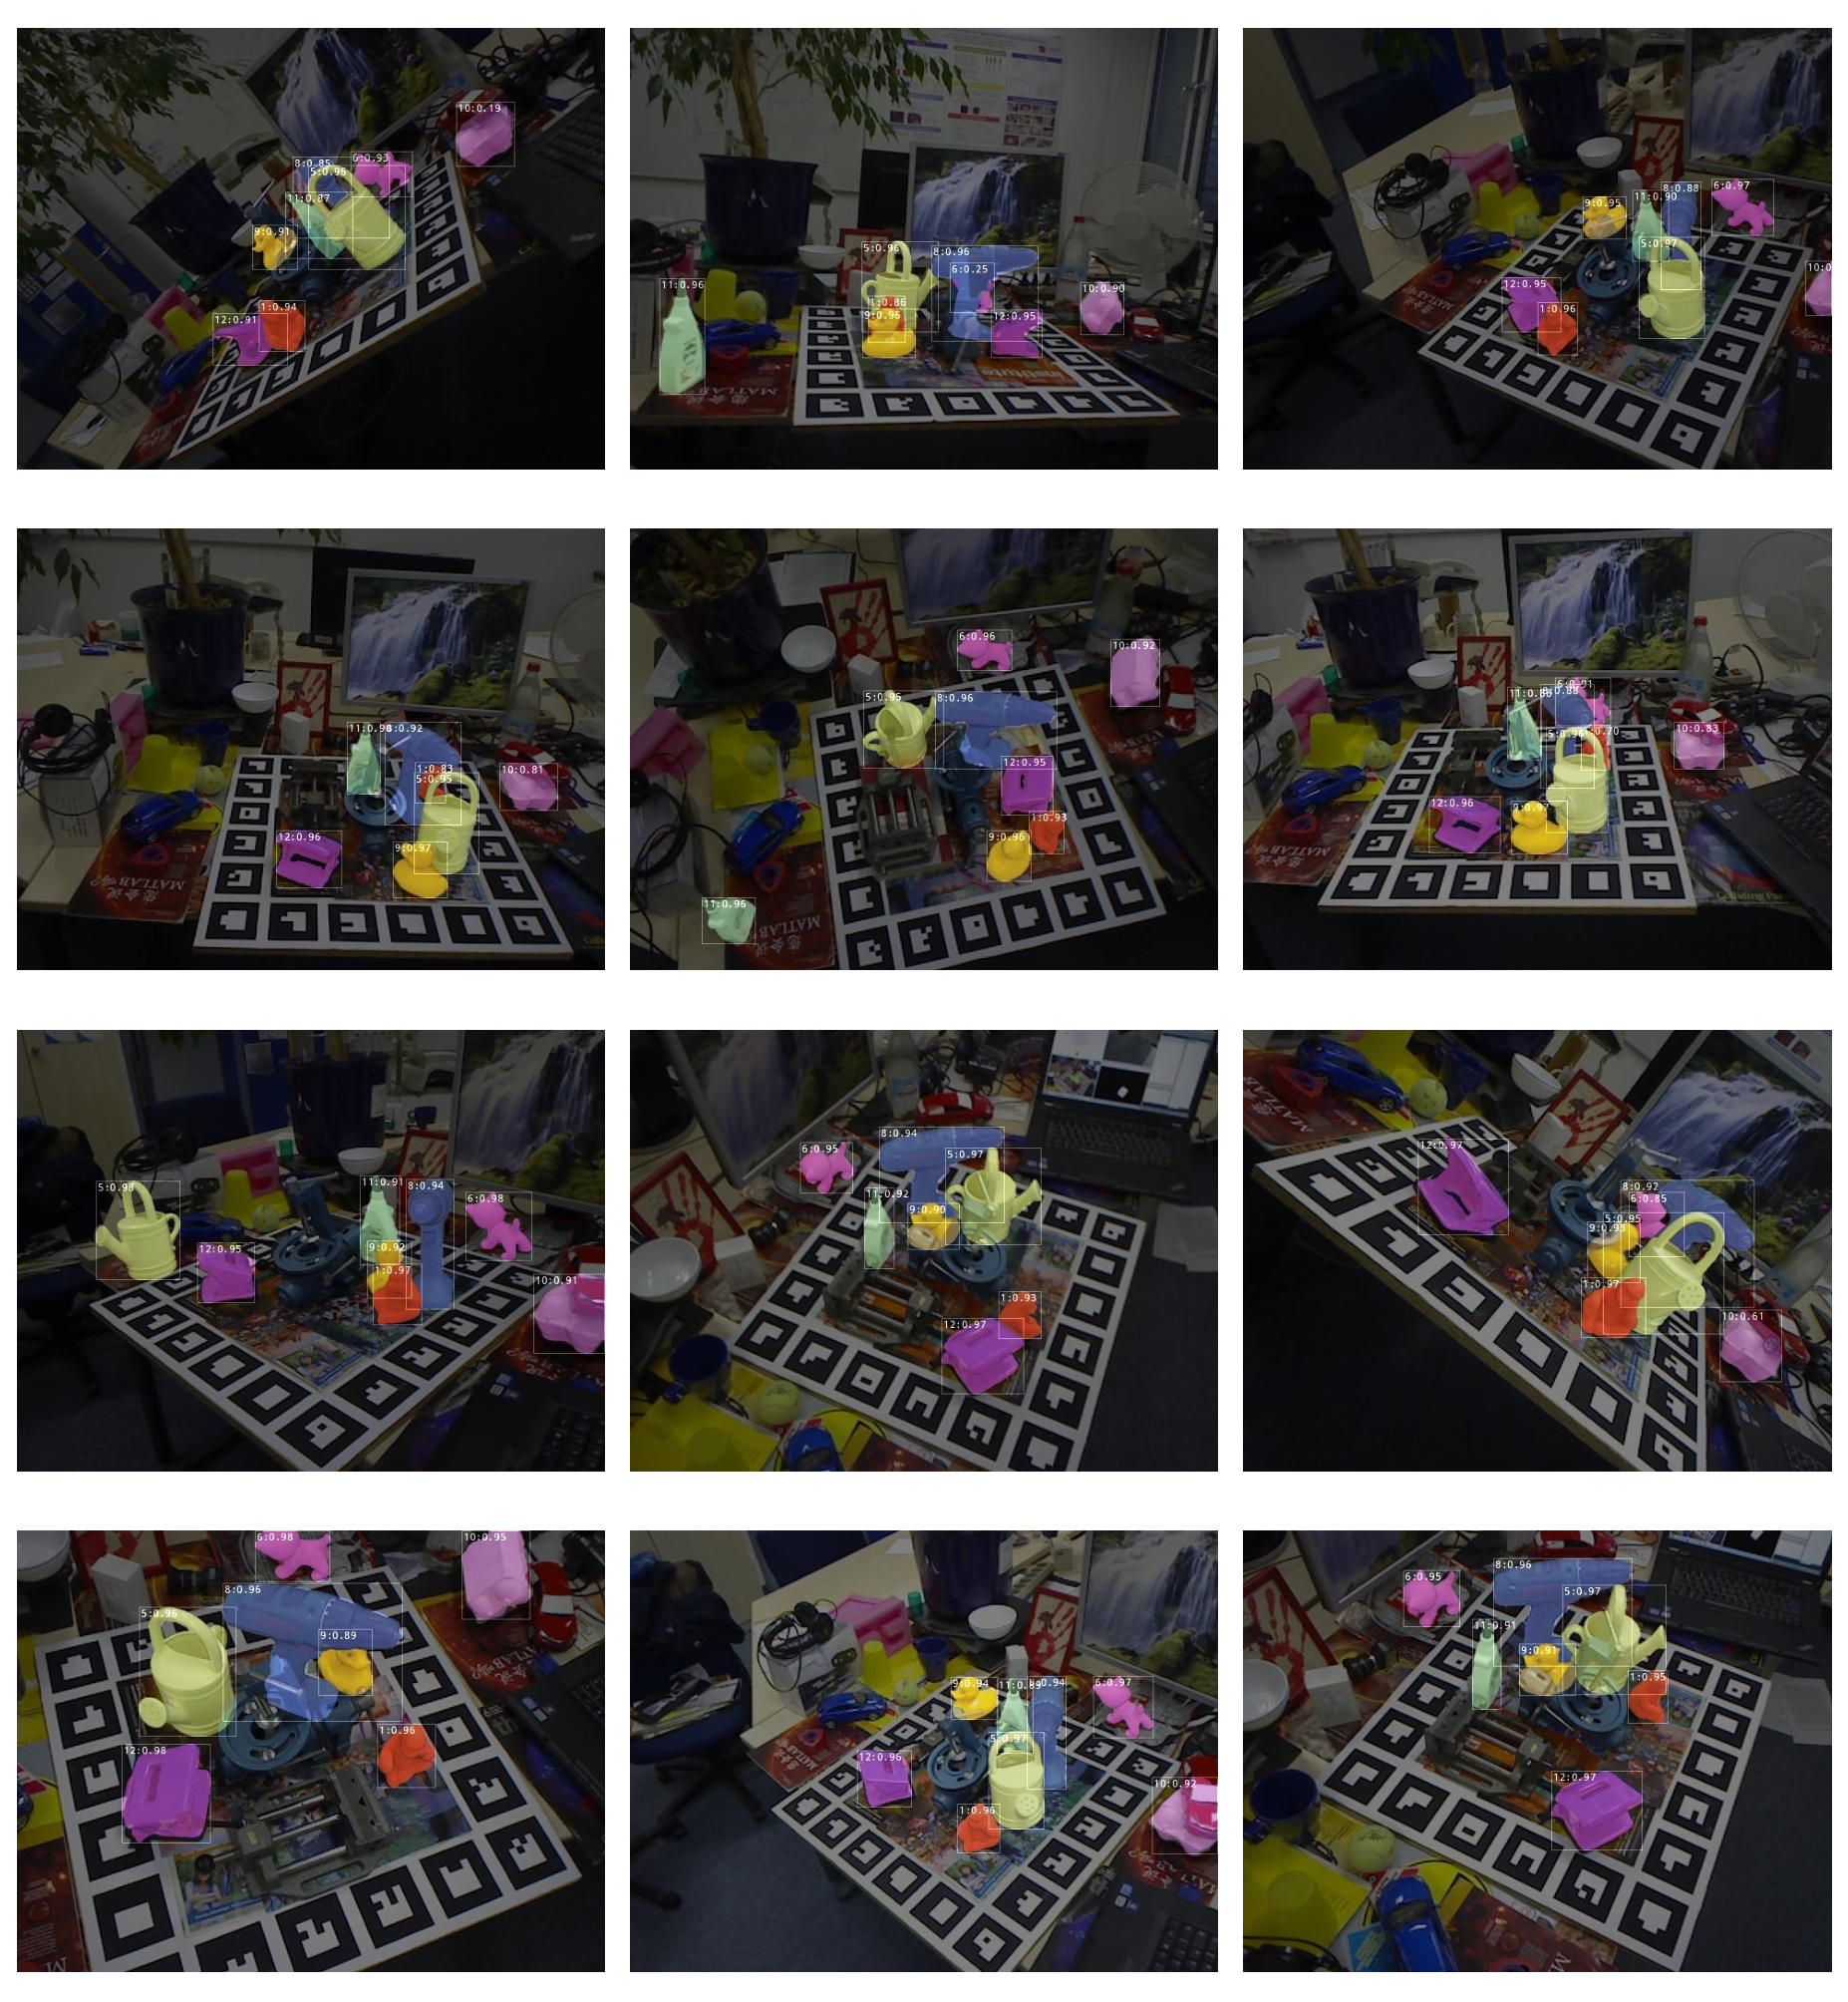
\includegraphics[width=1\linewidth]{figure/hipose/lmo_visulize.pdf}
    \caption{LM-O数据集可视化结果}
    \label{fig:Qualitative_LMO}
\end{figure}

\begin{figure}
    \centering
    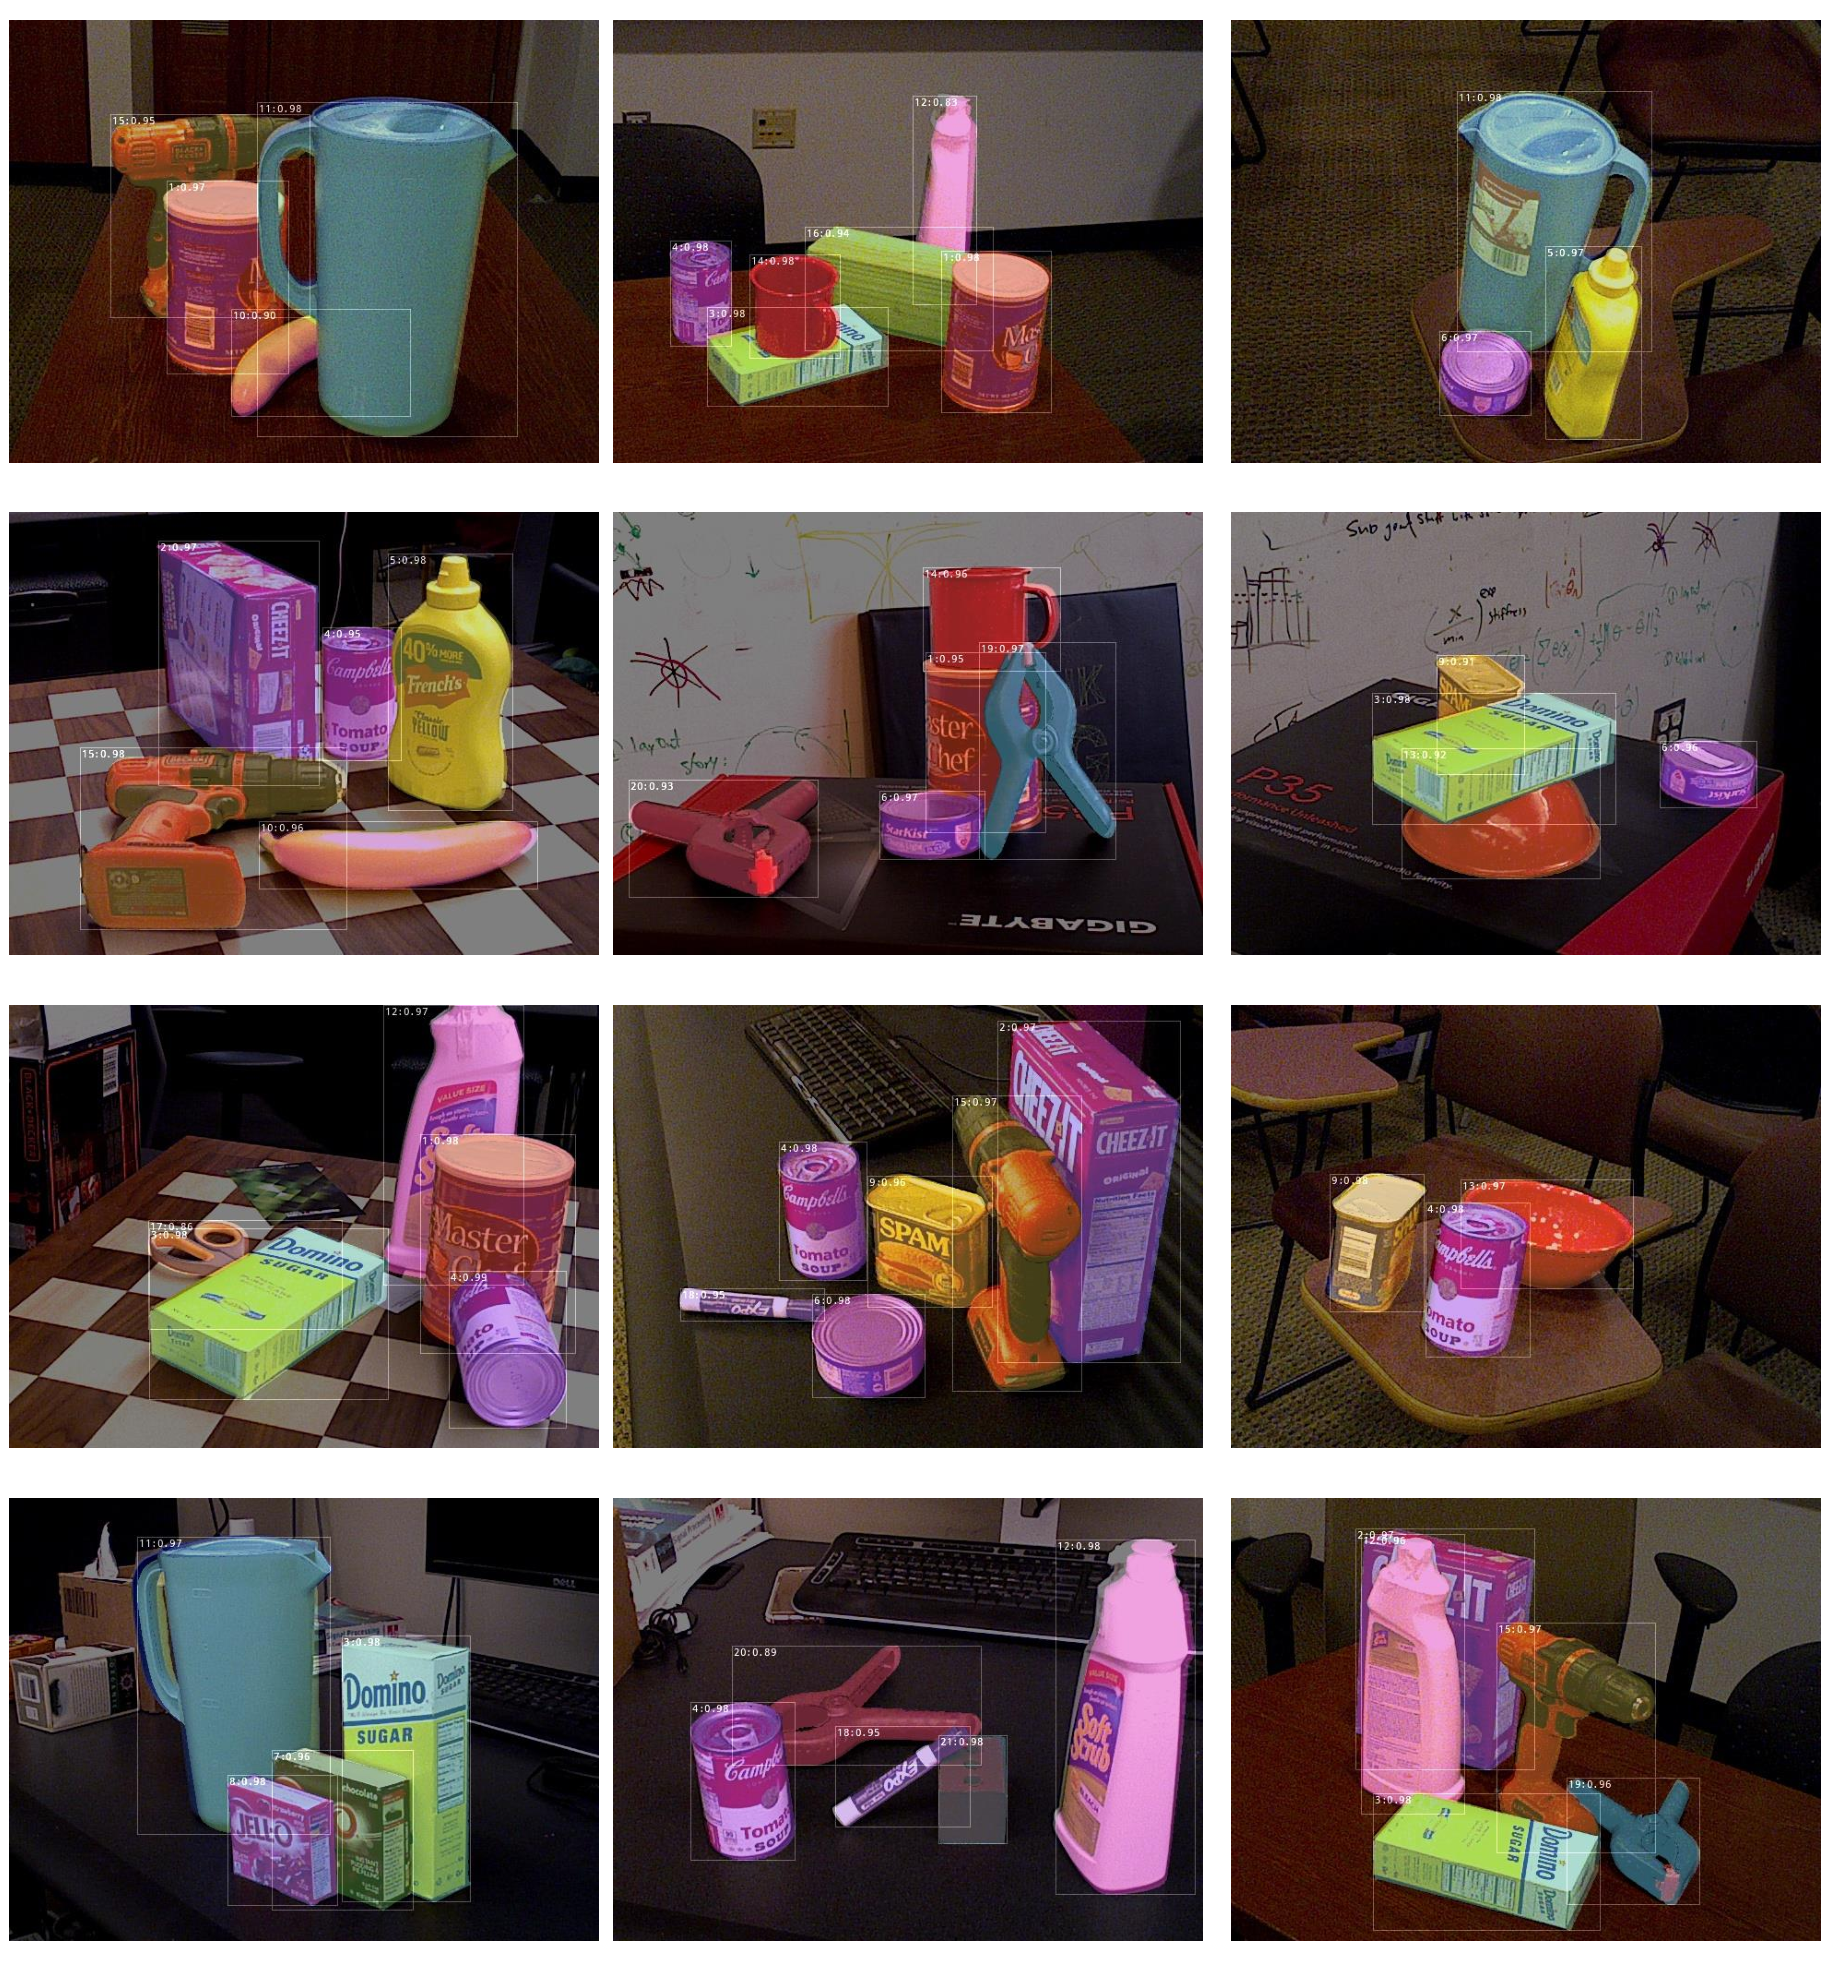
\includegraphics[width=1\linewidth]{figure/hipose/ycbv_visulize.pdf}
    \caption{YCB-V数据集可视化结果}
    \label{fig:Qualitative_YCBV}
\end{figure}

\begin{figure}
    \centering
    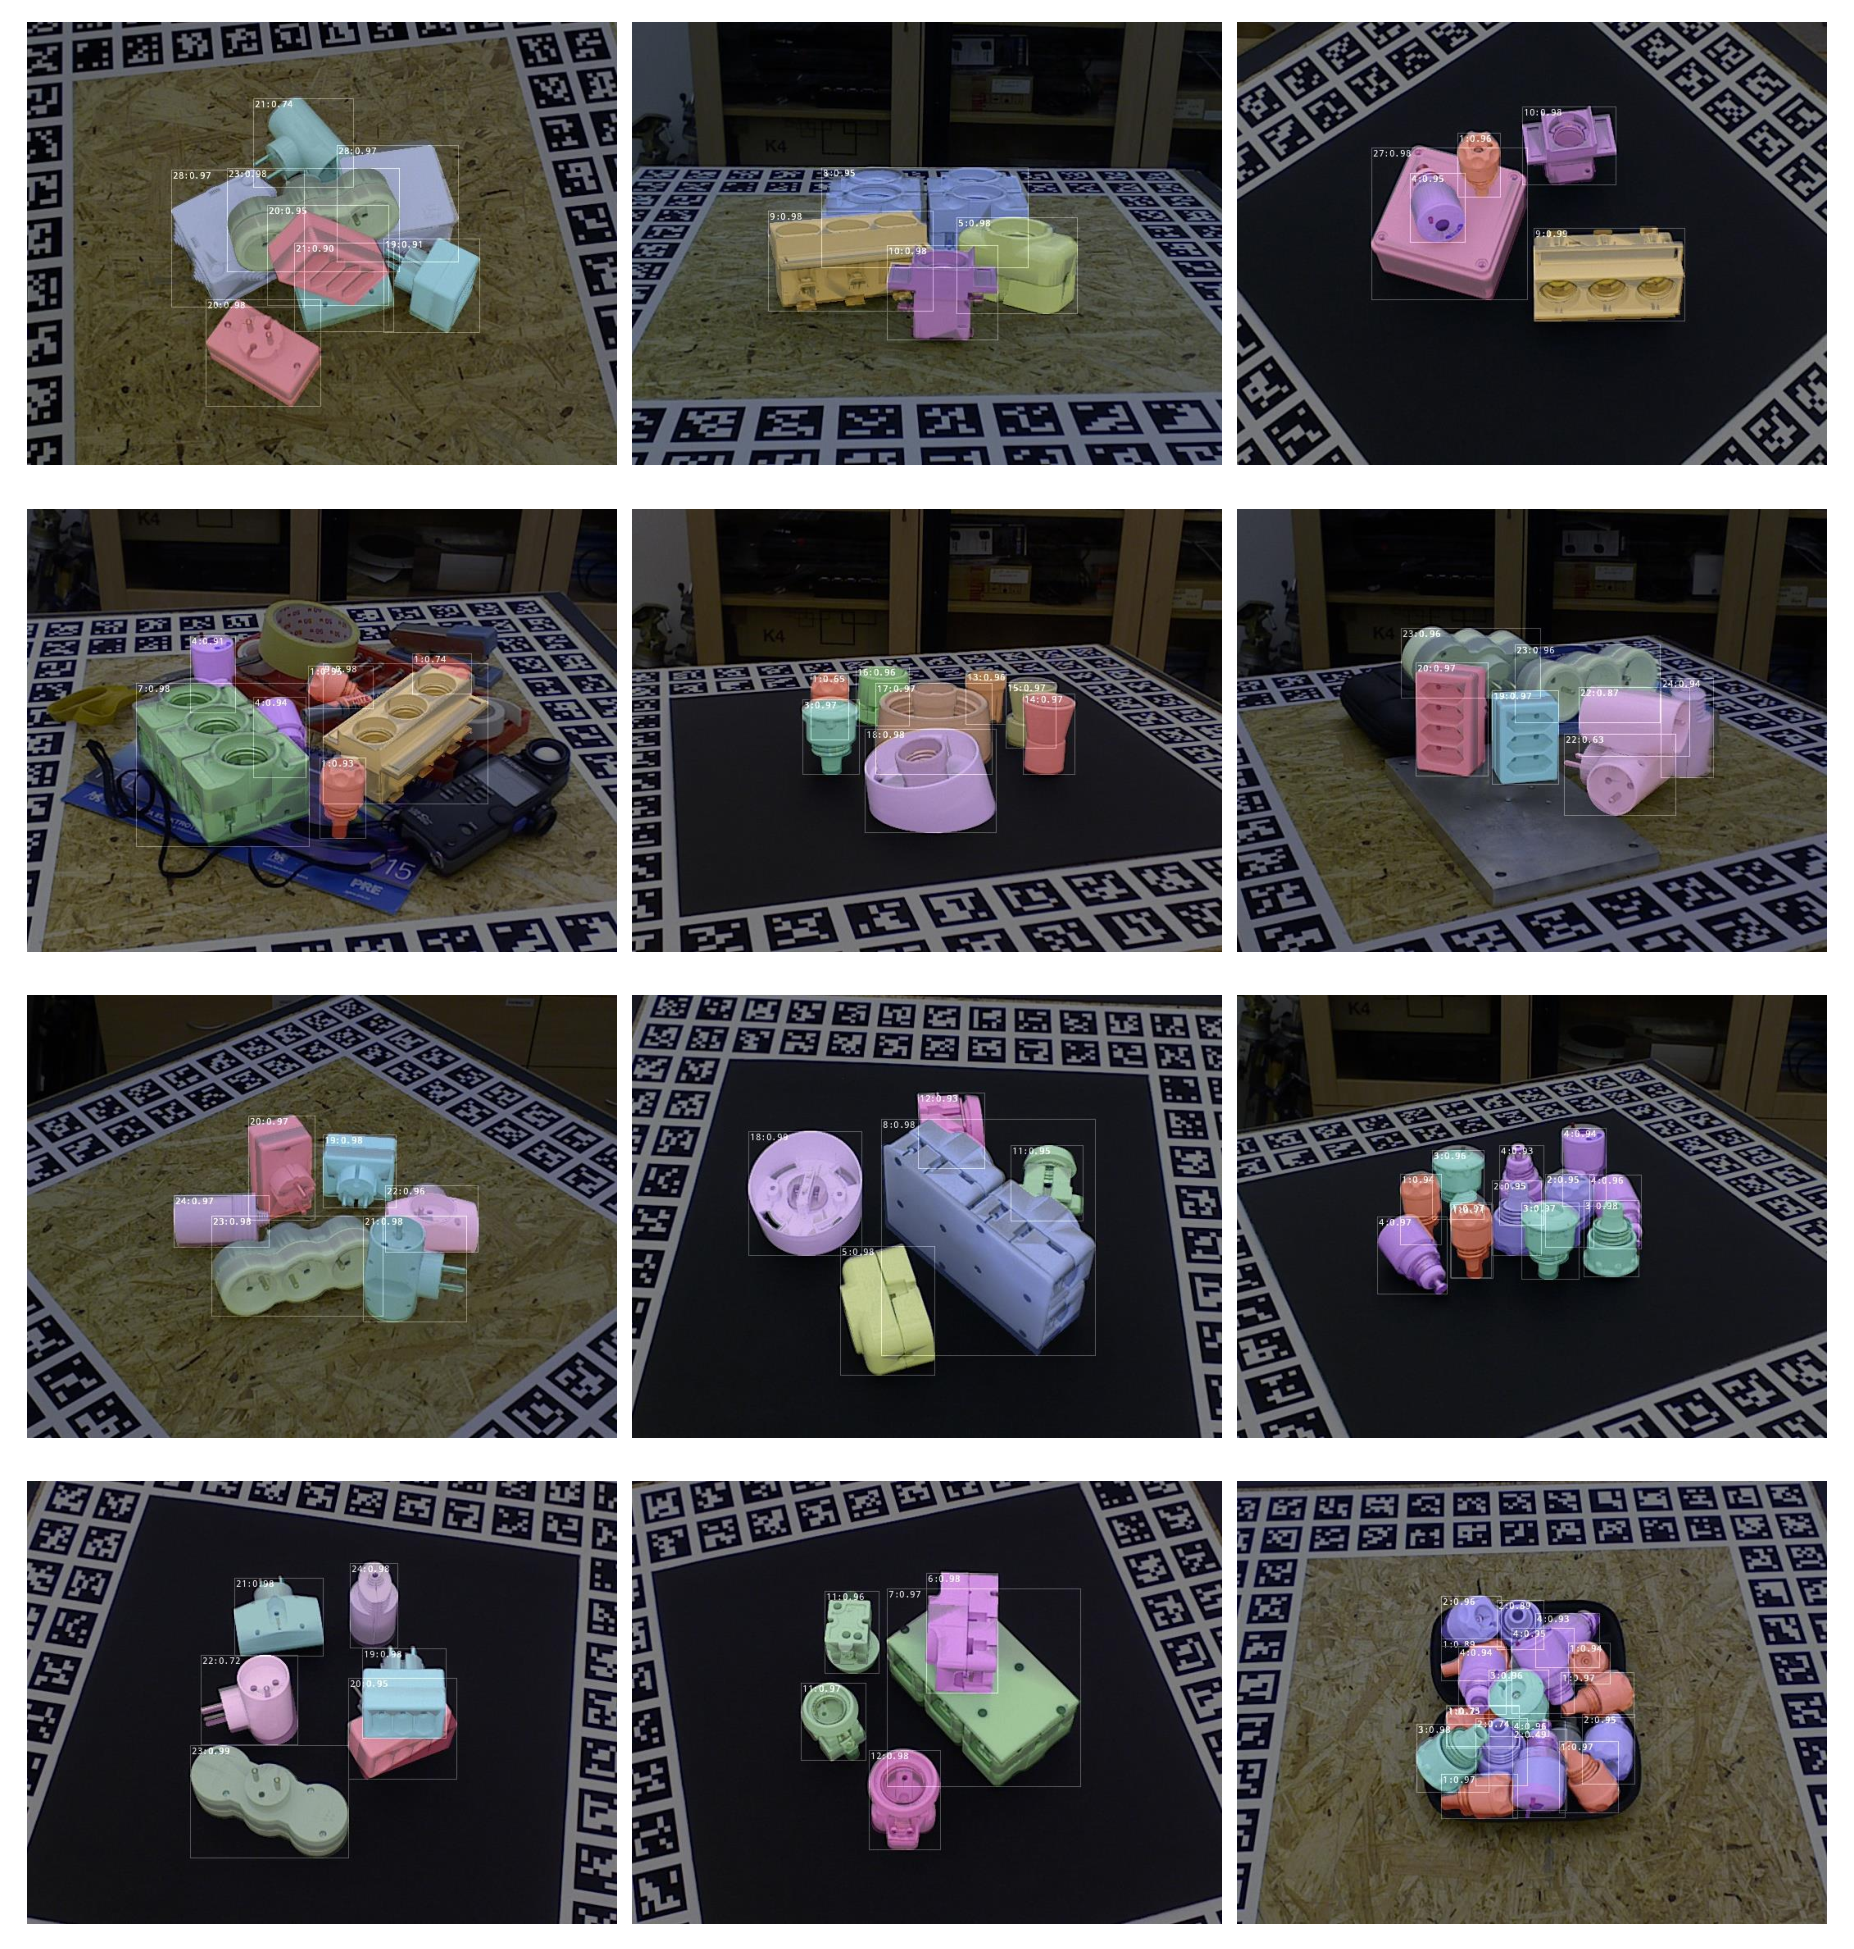
\includegraphics[width=1\linewidth]{figure/hipose/tless_visulize.pdf}
    \caption{T-LESS数据集可视化结果}
    \label{fig:Qualitative_TLESS}
\end{figure}

\begin{figure}
  \centering
  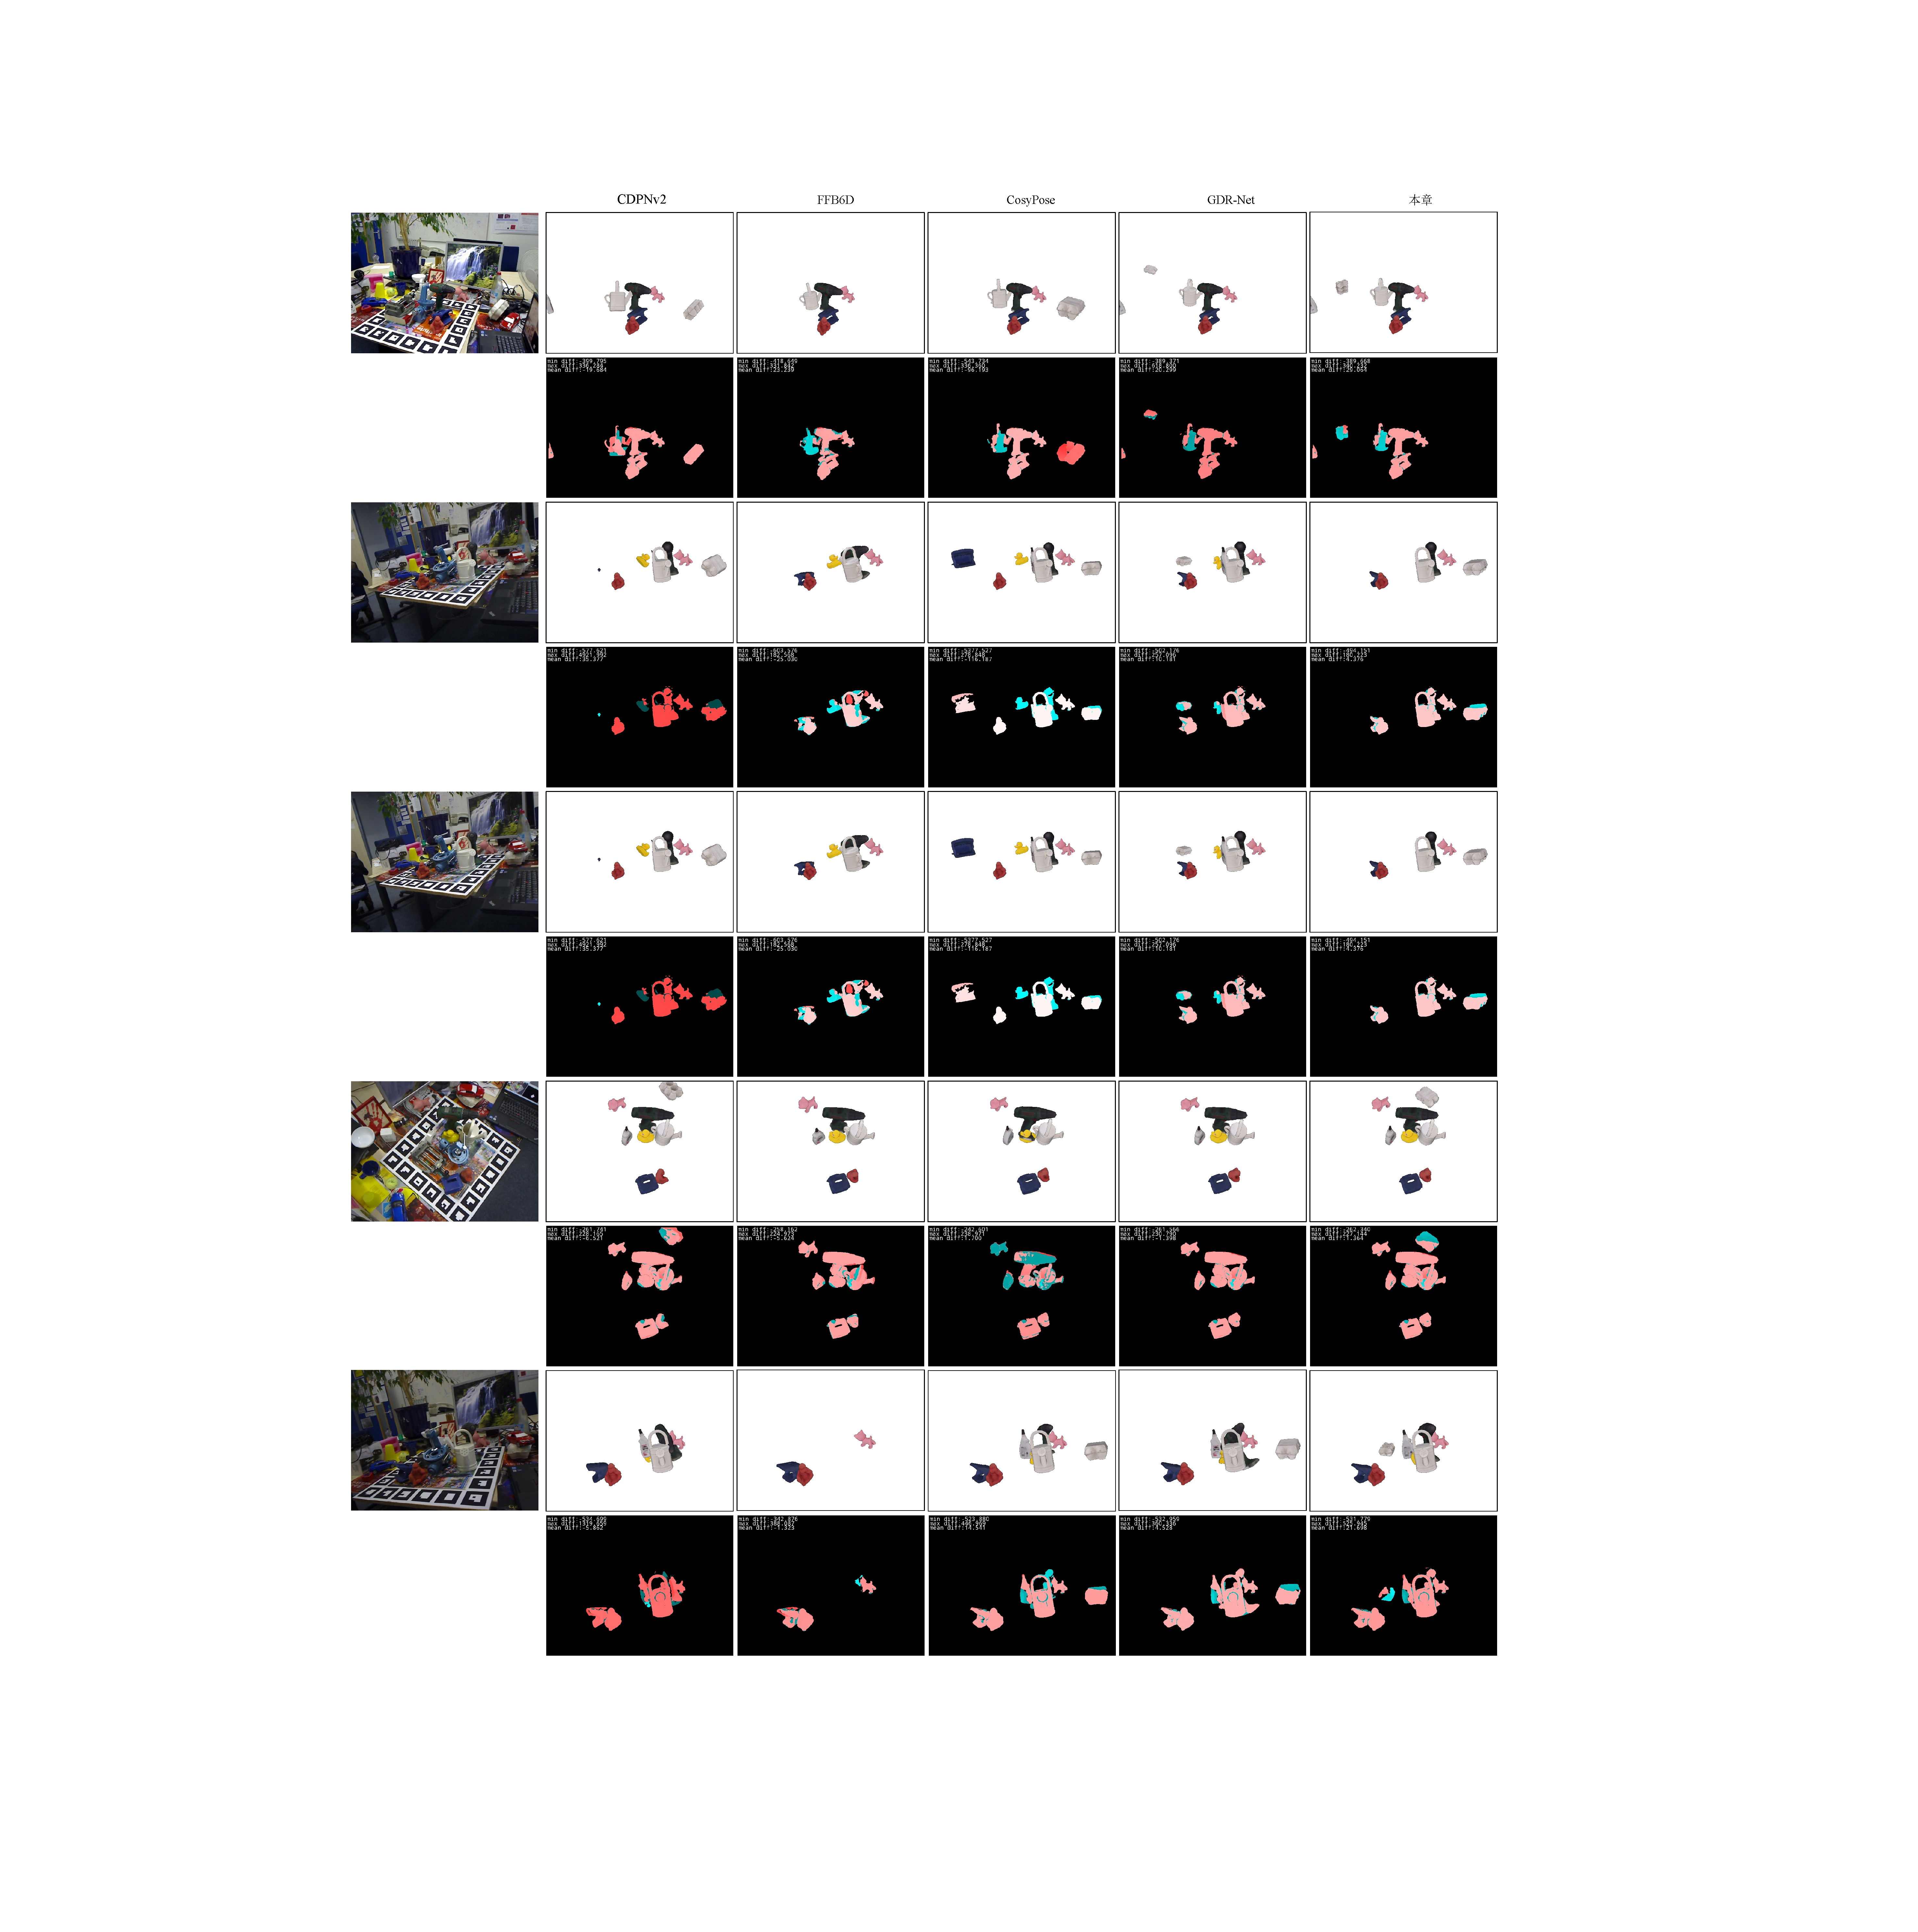
\includegraphics[width=1\linewidth]{figure/hipose/compare_visualize.pdf}
  \caption{不同方法对比可视化结果}
  \label{fig:Qualitative_different_methods}
\end{figure}